\documentclass[onecolumn]{article}
\usepackage{fancyhdr}
\usepackage{pgf}
\usepackage{multicol}
\usepackage{amsmath}
\usepackage{enumerate}
\usepackage{listings}
\usepackage[top=2in, bottom=1.5in, left=1in, right=1in]{geometry}
\usepackage{graphicx}
\usepackage{tabularx} 
\usepackage{url}

\lstset{
	tabsize=4,
        basicstyle=\scriptsize,
        aboveskip={1.5\baselineskip},
        columns=fixed,
        showstringspaces=false,
        breaklines=true,
        prebreak = \raisebox{0ex}[0ex][0ex]{\ensuremath{\hookleftarrow}},
	frame=none,
        showtabs=false,
        showspaces=false,
        showstringspaces=false,
        identifierstyle=\ttfamily,
        keywordstyle=\color[rgb]{0,0,1},
        commentstyle=\color[rgb]{0.133,0.545,0.133},
        stringstyle=\color[rgb]{0.627,0.126,0.941},
	language=C++
}

\def\SUBJECT{ECE 510}
\def\TOPIC{Final Project Proposal\\ \small{Z80 Core with Gameboy Extensions}}
\def\AUTHOR{Bradon \textsc{Kanyid} \\ Eric \textsc{Krause} \\ Tyler \textsc{Tricker}}
\def\INSTRUCTOR{Mark \textsc{Faust}}

%*******************Page layout
\pagestyle{fancy}
\lhead{\AUTHOR}
\chead{\SUBJECT: \TOPIC}
\rhead{\thepage}
\fancyfoot{}


\begin{document}
\begin{titlepage}
 \begin{center}
 \newcommand{\HRule}{\rule{\linewidth}{0.5mm}}
% Upper part of the page. The '~' is needed because \\
% only works if a paragraph has started.

\textsc{\LARGE Portland State University}\\[1.5cm]

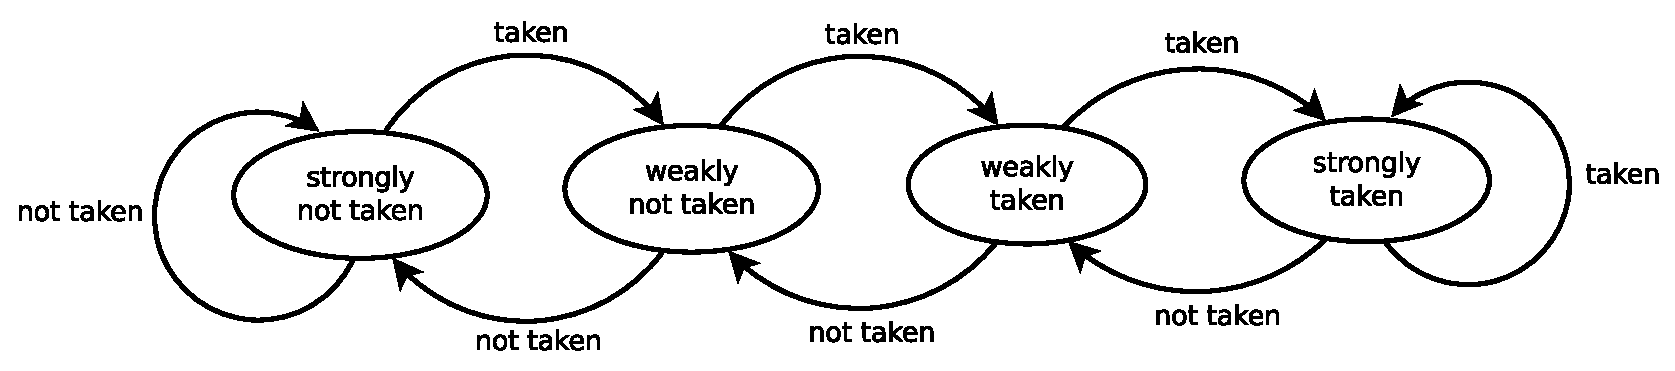
\includegraphics[width=0.5\textwidth]{../latex_common/logo}~\\[1cm]

\textsc{\Large \SUBJECT}\\[0.5cm]

% Title
\HRule \\[0.4cm]
{ \huge \bfseries \TOPIC}\\[0.4cm]

\HRule \\[1.5cm]

% Author and supervisor
\begin{minipage}{0.4\textwidth}
\begin{flushleft} \large
\emph{Author:}\\
\AUTHOR
\end{flushleft}
\end{minipage}
\begin{minipage}{0.4\textwidth}
\begin{flushright} \large
\emph{Instructor:} \\
\INSTRUCTOR
\end{flushright}
\end{minipage}

\vfill

% Bottom of the page
{\large \today}

\end{center}

\end{titlepage}


\section{Introduction}
This project does lots of awesome things with System Verilog and neat stuff.

\subsection{Branch Target Prediction}
\subsection{Branch Target Buffer}


\section{Project Focus}
Our project will focus on the CPU core of a gameboy using a previous project,
FPGABOY \footnote{FPGABOY - an implementation of a gameboy system onto an FPGA 
writen in Verilog}. Another team will be focusing on peripherals for our project 
so that they can operate as a complete system. The CPU core, originally writen 
in Verilog, will be ported to use a synthesizable subset of System Verilog.
The synthesis target we will be focusing on will be on an Altera Cyclone II 
FPGA kit available in FAB 60-04\footnote{Part Number DK-CYCII-2C20N}.

Testing will use two modes from the Veloce Solo tools; the synthesizeable 
testbench and the TBX modes. For testbench data, there are test ROMs created 
for testing gameboy emulators, which we can use to verify that our instruction 
set simulation is accurate. There are also timing tests within the test ROMs. 

For additional tests, we will be able to create test programs using the GBDK development kit and Gameboy assembler.



\section{Resources}
\begin{itemize}
    \item {\bf Fpgaboy}
            - Main website for Verilog implementation\\
            {\it fpgb.org} \\
            {\it github.com/trun/fpgaboy}
    \item {\bf Pandocs} - Reversed-engineered hardware documentation\\ 
            {\it nocash.emubase.de/pandocs.htm}
    \item {\bf Quartus II Web Edition} - System Verilog toolset 
             for synthesis analysis and final project synthesis\\
            {\it altera.com/products/software/quartus-ii/web-edition/qts-we-index.html}
    \item {\bf Mentor Graphics Veloce} - System Verilog implementation and simulation hardware\\
            {\it mentor.com/products/fv/emulation-systems/veloce}
    \item {\bf Game Boy Test Roms}     - Test images for compliance testing\\
            {\it gbdev.gg8.se/wiki/articles/Test\_ROMs}
    \item {\bf Game Boy Tool Chain} - For low-level C code testing\\
            {\it gbdev.gg8.se/wiki/articles/GBDK}
    \item {\bf Z80 Assembly Programming Tutorial} - Sample code to compile and test\\
            {\it cratel.wichita.edu/cratel/ECE238Spr08}
    \item {\bf Project Repository}\\
            {\it github.com/rattboi/gateboy}
    \item {\bf Project Wiki}\\
            {\it github.com/rattboi/gateboy/wiki}
\end{itemize}



\end{document}
